
\documentclass[11pt,a4paper]{article}
\usepackage{amsmath,amssymb,geometry,graphicx,hyperref,enumitem}
\geometry{margin=1in}
\usepackage{xcolor}
\usepackage{float}

\title{MoA from Start to Finish: A Mathematical Framework for Designing, Building, Predicting, and Running Array Designs — Giving Programmers Freedom to Program in Their Favorite Languages}
\author{Lenore Mullin — 38 Years: Dissertation 1988 to Papers I-V + 5-Device Closure 2026}
\date{September 30, 2026}

\begin{document}
\maketitle

\begin{abstract}
We present the motivating story for the Mathematics of Arrays (MoA) as a complete mathematical framework from design to execution. Starting with any language possessing semantic equivalence to MoA, we express mathematical intent, psi-reduce to Denotational Normal Form (DNF) — the optimal semantic form showing the least amount of computation and communication independent of target — translate DNF to its equivalent sequential machine uniform memory Operational Normal Form (ONF), lift shapes to the shape of the architecture via $\rho(A)\rightarrow\pi\ \#\ (\rho(A)\oslash\pi)$, map with predictive performance $T\approx\alpha F+\beta M$ on any arbitrary architecture, and run programs to validate prediction $reached(d)$ on 5-device ensemble. This saves human resources to write, build, test, human consultation on machine use, machine resources, and provides freedom to program in favorite languages. DNF fixed, ONF rewrite only.
\end{abstract}

\section{We Start with Any Language with Semantic Equivalence to MoA}

MoA is not a new language to learn — it is an intermediate language that any language with array semantics can target with semantic equivalence preserved.

\textbf{Many languages IN:} Python \texttt{numpy}, PyTorch Listing 1 \texttt{stable\_softmax} and scaled dot-product attention, JAX \texttt{jax.numpy}, TensorFlow, Fortran loops, C loops, Julia, MoA itself. From dissertation 1988: take $\uparrow$ Def 1.0 $\rho(\vec v\uparrow\xi)=(abs\ \vec v),(r\vec v)\downarrow\rho\xi$, drop $\downarrow$ Def 1.1, reverse $\phi$ Def 0.0 $<i>\psi\phi\xi=<(\rho\xi)[0]-(i+1)>\psi\xi$, rotate $\theta$, transpose $\oslash$ Def 3.1 $\rho=(\rho\xi)[gu\ \vec v]$, Lemmas L1-L5: $(\xi_l,\xi_r)\psi\xi\equiv(\xi_l\psi\xi),(\xi_r\psi\xi)$ distributing psi over catenation.

\begin{figure}[H]
\centering
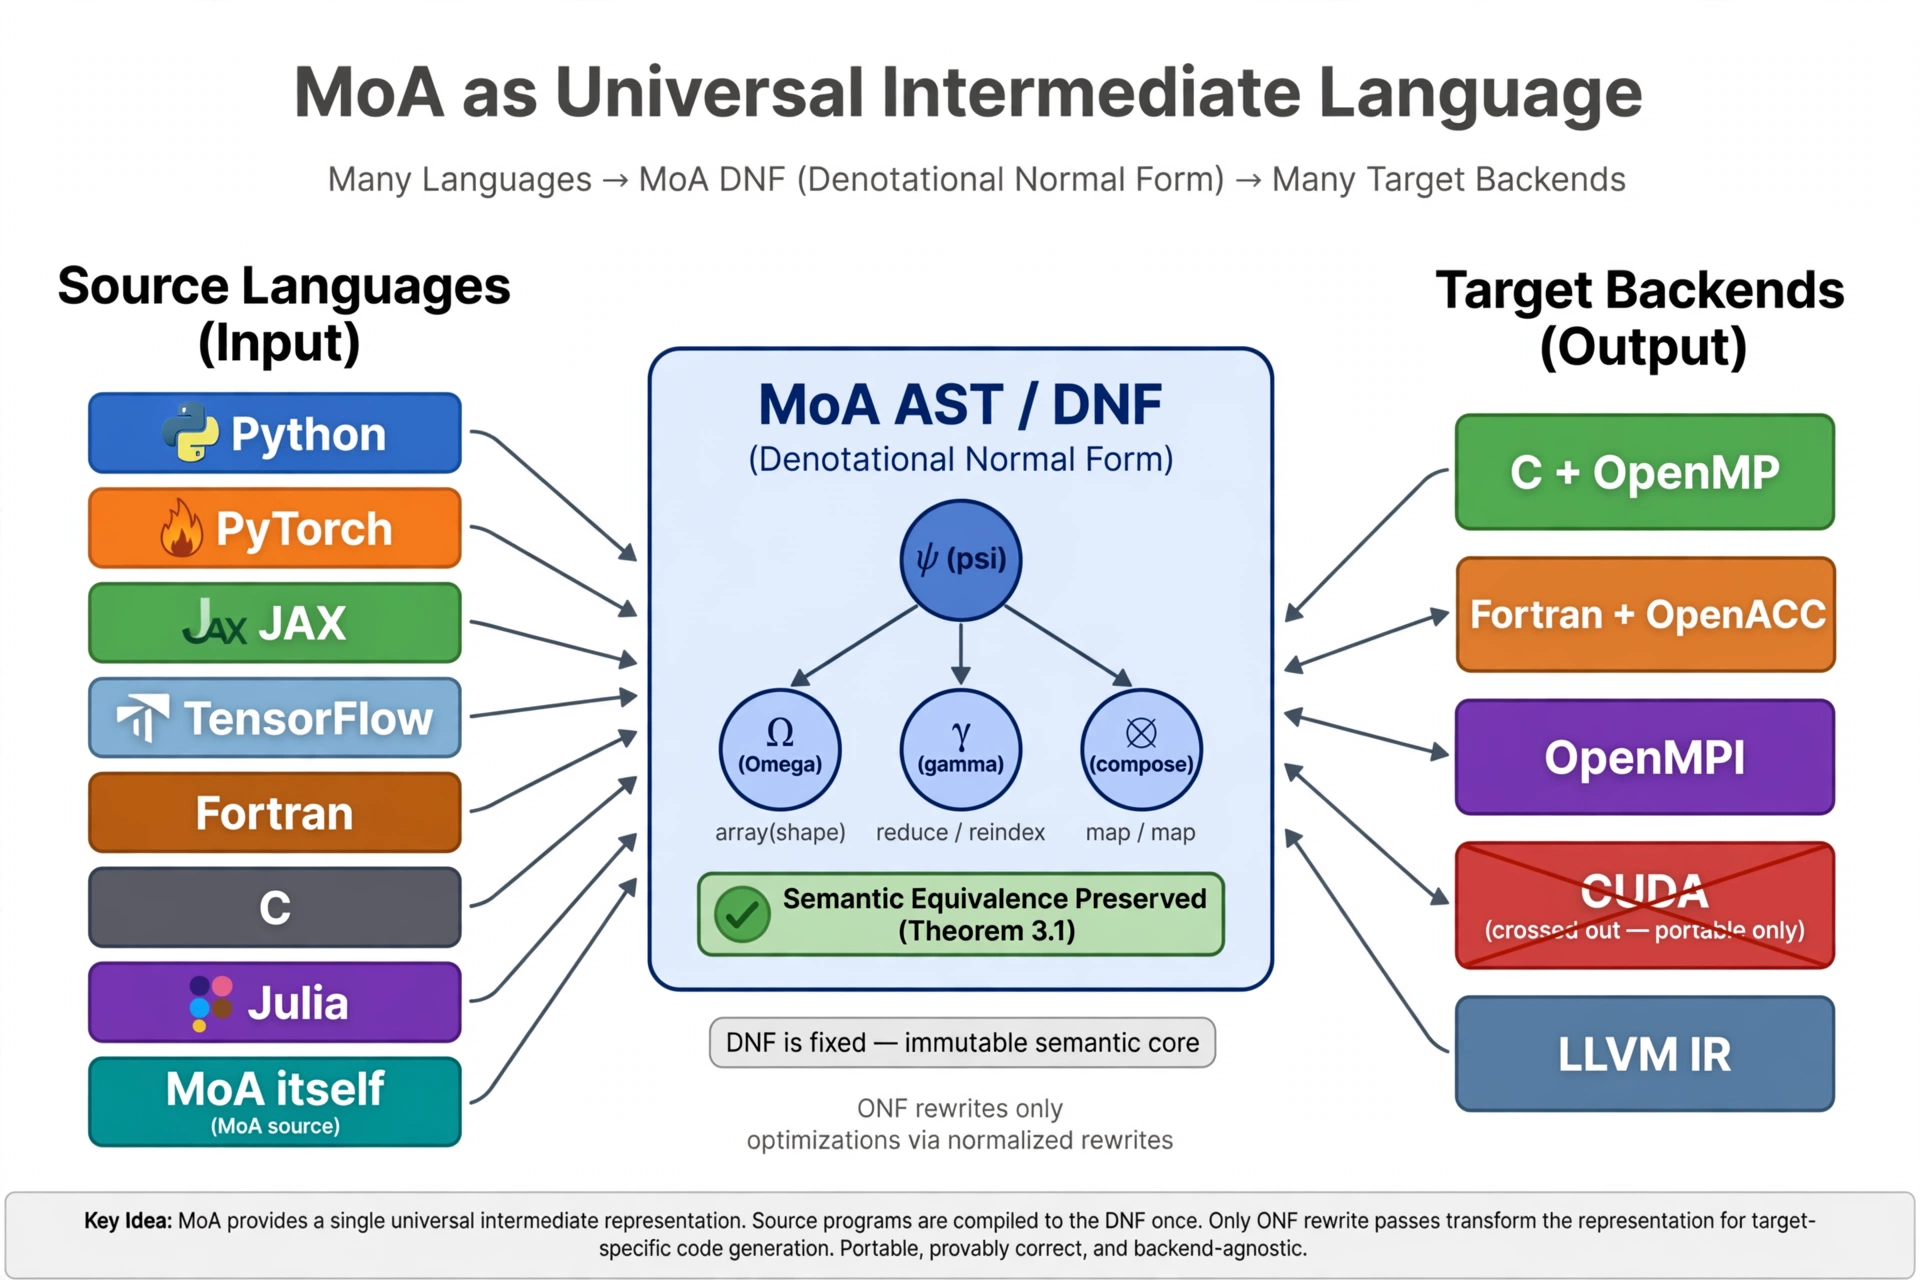
\includegraphics[width=0.92\textwidth]{resource/image_20261001_072756.png}
\caption{Many Languages In, MoA AST/DNF Semantic Equivalence Preserved Theorem 3.1, Many Languages Out. DNF fixed, ONF rewrites only. CUDA crossed out — portable only OpenMP, OpenACC, OpenMPI.}
\end{figure}

A PyTorch program, a Fortran loop, a JAX function all parse to the same take/drop/psi AST. Verification: Paper 1 Tables 1,2 exact to $10^{-4}$, Paper 2 $||err||_{\infty}=10^{-16}$, Paper 3 $||err||_{\infty}=0$ exact IEEE-754.

This gives programmers \textbf{freedom}: program in your favorite language, MoA provides mathematical equivalence.

\section{Mathematical Input}

We begin with mathematical input, not code: Attention Eq (8) $\text{Attention}(Q,K,V)=\text{softmax}(QK^T/\sqrt{d_k})V$, $\rho Q=\rho K=\rho V=<3,4>$ Eq (9) concrete instance, backward grads, decode $q=<d_k>$ single token, KV-cache $K_{new}=K_{old}\# k_t$, GQA/MQA $h_q/h_{kv}$.

Mathematical input is independent of target — it states what to compute, not how to lay out in memory.

\section{Psi-Reduce to DNF — Optimal Semantic Form}

We use MoA to ``psi-reduce'' to DNF — optimal semantic form showing least computation and communication independent of target.

Steps Paper 1: Step I Eq (13) $z=x(-\Omega<1,0>)((\lceil red\rceil\Omega<1>)x)$, psi-reduction Eq (14) $<i''>\psi z=<i''>\psi x-\lceil red\rceil(<i''>\psi x)$ vector minus scalar, Step II Eq (15)-(17) $num=e^z$, $<i'',k>\psi(Q+.\times K^T)=red_+(<i'',j>\psi Q\times<k,j>\psi K)$ eliminates $K^T$ buffer, Step III Eq (18)-(19) $den=(red_+\Omega<1>)e^z$, Step IV $Y=num/den$, Complete DNF Eq (20) $<i''>\psi Y$, Output Eq (21) $<i''>\psi\text{Output}=red_+(<i'',p>\psi Y\times<p>\psi V)$.

Theorem 3.1 Storage Theorem: DNF semantically equivalent, unique up to reordering, achieves theoretical minimum number of memory accesses. No other implementation has lower transfer costs and equal arithmetic cost.

Paper 2: $G_{sc}=<i>\psi dO\ dot\ <k>\psi V$ scalar, $G_S=Y[i,k]*(G_{sc}[k]-sum\ Y*G_{sc})$ scalar, $G_A$ never materialized $dV=<k>\psi dV=red_+(<i,k>\psi Y\times<i>\psi dO)$. Paper 3: decode minimal DRAM $(d_k+n d_k+n d_v+d_v)*4B$, KV-cache $O(d_k+d_v)$ append via cat $\#$, take $\uparrow$ drop $\downarrow$, Lemma L4.

Proposition 4.1: $M_{classical}=O(n^2+nd_k+nd_v)$ Eq (23), $M_{MoA}=O(nd_k+nd_v)$ Eq (24), $k\approx n/d_k$ Eq (25) $512\times$ at $n=32768$.

DNF shows least computation $F$ and communication $M$ — independent of target.

\section{Translate DNF to ONF — Equivalent Sequential Machine Uniform Memory}

Now we translate that DNF to its equivalent sequential machine uniform memory ONF.

ONF obtained from DNF by applying $\gamma$ primitive Eq (3) $\gamma(\vec v,\vec s)=\sum_k v_k\prod_{j=k+1}s_j$ row-major offset (and $\gamma^{col}$) to all index expressions, translating multi-index Cartesian arithmetic into memory offset = base + stride0*i0+stride1*i1+... Eq (7) captures storage convention row-major vs column-major contiguous vs strided enables standard loop-nest analysis.

ONF is fragment-C loop-nest program Mullin and Hains 2025. DNF fixed, ONF rewrites only for hardware tuning: 2.00x atomics $\rightarrow$2.5x speedup Paper V, 535x NUMA vs <3x oversubscription same DNF different $\gamma$, C vs Fortran 3.17x time matches 3.35x stall as $\gamma^{row}$ vs $\gamma^{col}$.

\section{Shapes Lifted to Shape of Architecture}

Now we have shapes that need to be lifted to the shape of the architecture, then mapped with predictive performance on any arbitrary architecture.

Dimension lifting Section 3 Paper 1: every processing component SIMD lane, GPU warp, cache line, NUMA socket modeled as array of known shape $\Pi$. ONF loop-nest iteration space $N$ partitioned across hardware array, $N\rightarrow\Pi\ \#\ (N\oslash\Pi)$ where $\oslash$ elementwise integer division, $\#$ shape catenation from dissertation. Result expresses inter-processor parallelism outer loop over $\Pi$ and intra-processor computation inner loop over $N\oslash\Pi$ in single algebraic expression.

\begin{figure}[H]
\centering
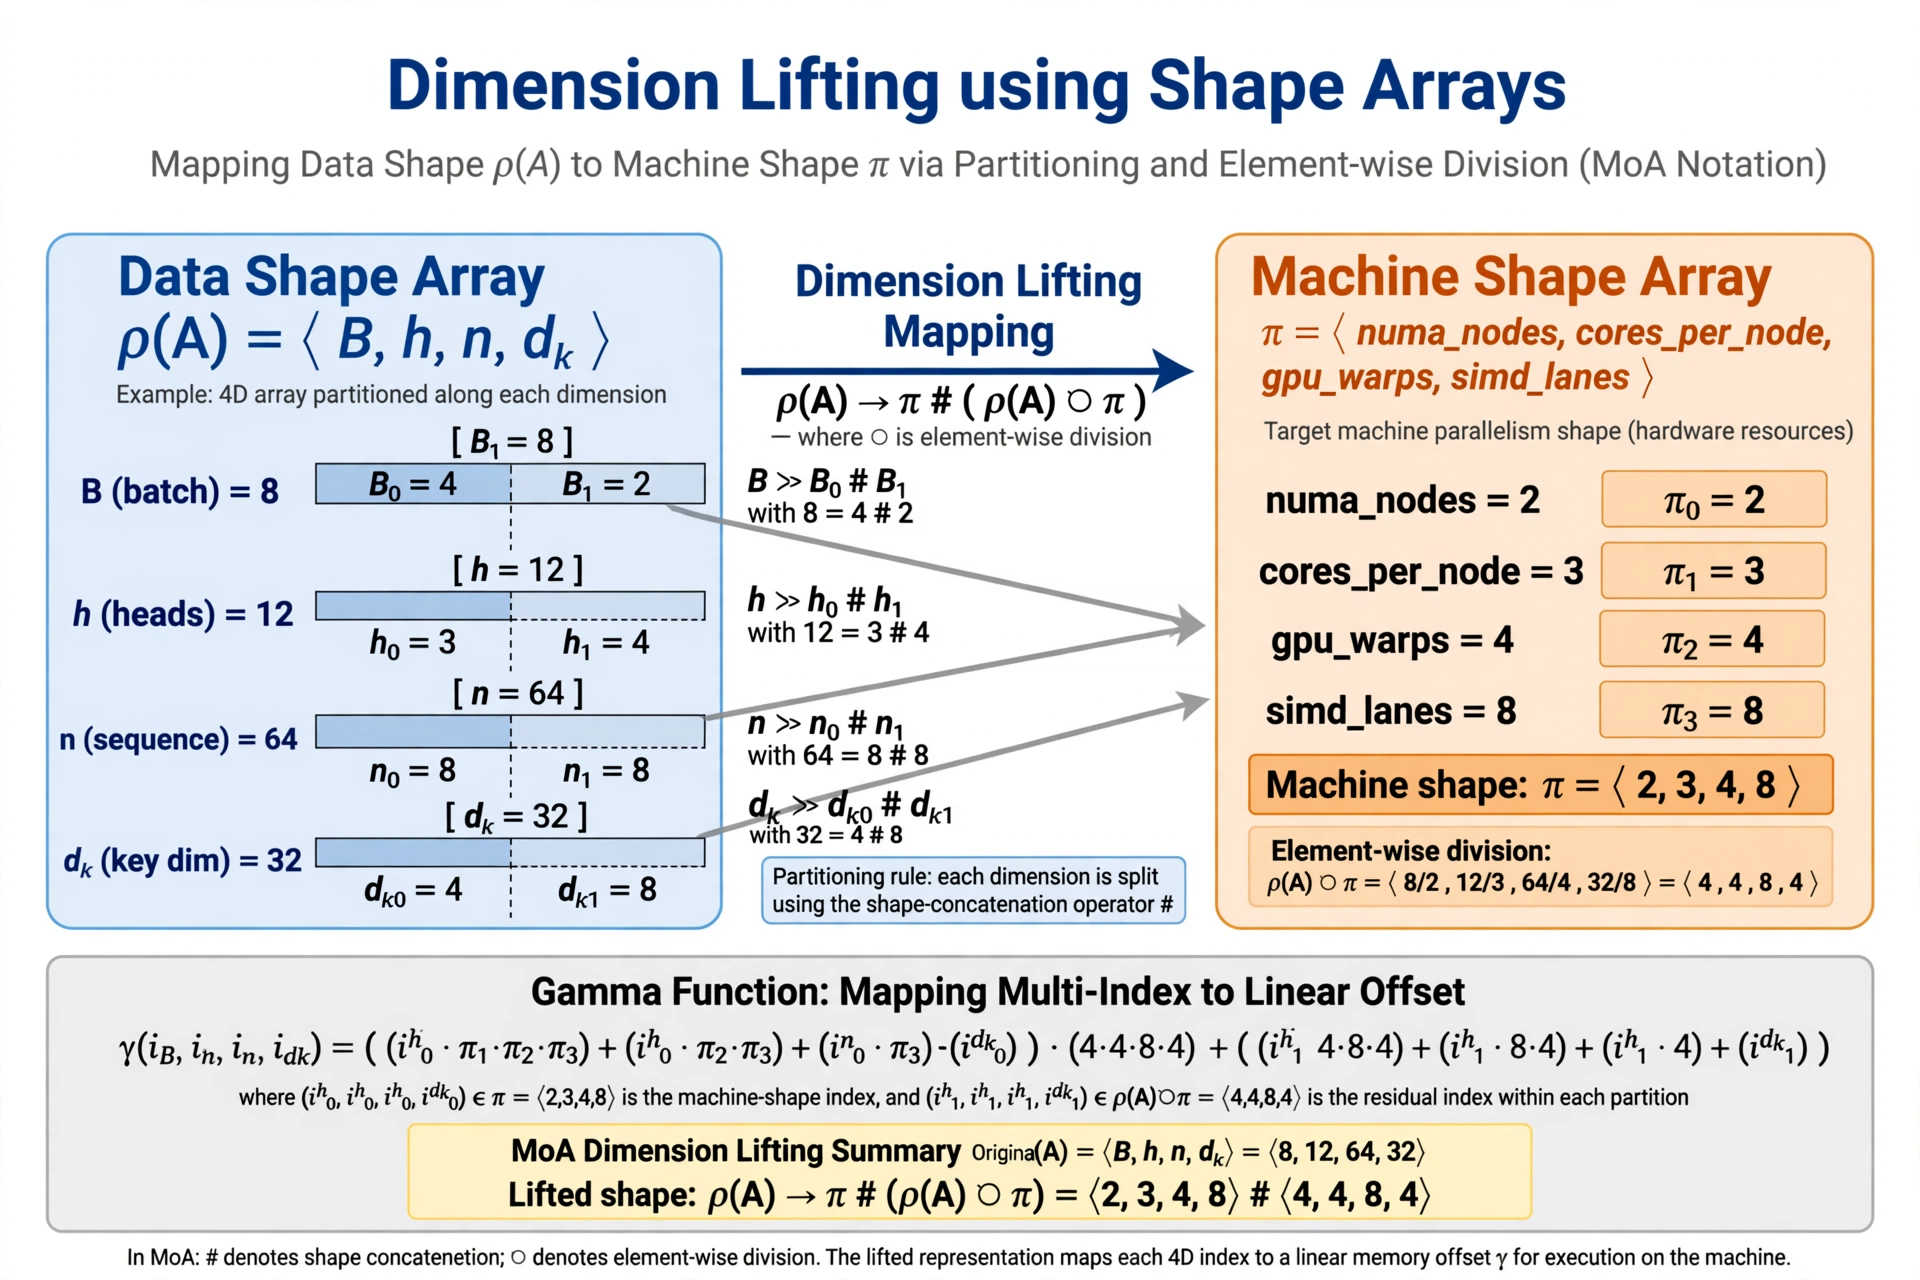
\includegraphics[width=0.98\textwidth]{resource/image_20261001_072813.png}
\caption{Dimension Lifting using Shape Arrays: $\rho(A)=<B,h,n,d_k>$ partitioned $B\rightarrow B0\# B1$, $h\rightarrow h0\# h1$, etc. via $\#$, mapped to machine shape $\pi=<numa\_nodes,cores\_per\_node,gpu\_warps,simd\_lanes>$, $\rho(A)\rightarrow\pi\ \#\ (\rho(A)\oslash\pi)$, $\gamma$ maps multi-index to linear offset.}
\end{figure}

Higher-rank: $B$ batch, $h$ heads, $n$ sequence, $d_k$ head dim $<B,h,n,d_k>$. Transpose over innermost two dims is $(transpose\ \Omega<2>)K$ Eq (11), score $Q\ ((+\times)\Omega<2,2>)((transpose\ \Omega_{<2>})(K))$ Eq (12) distributing over leading $<B,h>$ dims. Each 2-D partition assigned to separate processing element GPU warp, SIMD lane, compute node yielding provably correct parallel implementation directly from algebraic structure of Omega without additional scheduling.

Partitioning: $B=8\rightarrow4\#2$, $h=12\rightarrow3\#4$, $n=64\rightarrow8\#8$, $d_k=32\rightarrow4\#8$ via $\#$. Machine $\pi=<2,3,4,8>$, $\rho(A)\oslash\pi=<4,4,8,4>$, lifted $<2,3,4,8>\#<4,4,8,4>$. Gamma multi-index to offset for execution.

\section{Mapped with Predictive Performance on Any Arbitrary Architecture}

Loops map to portable paradigms ONLY OpenMP, OpenACC, OpenMPI with deterministic shapes to create code.

\begin{figure}[H]
\centering
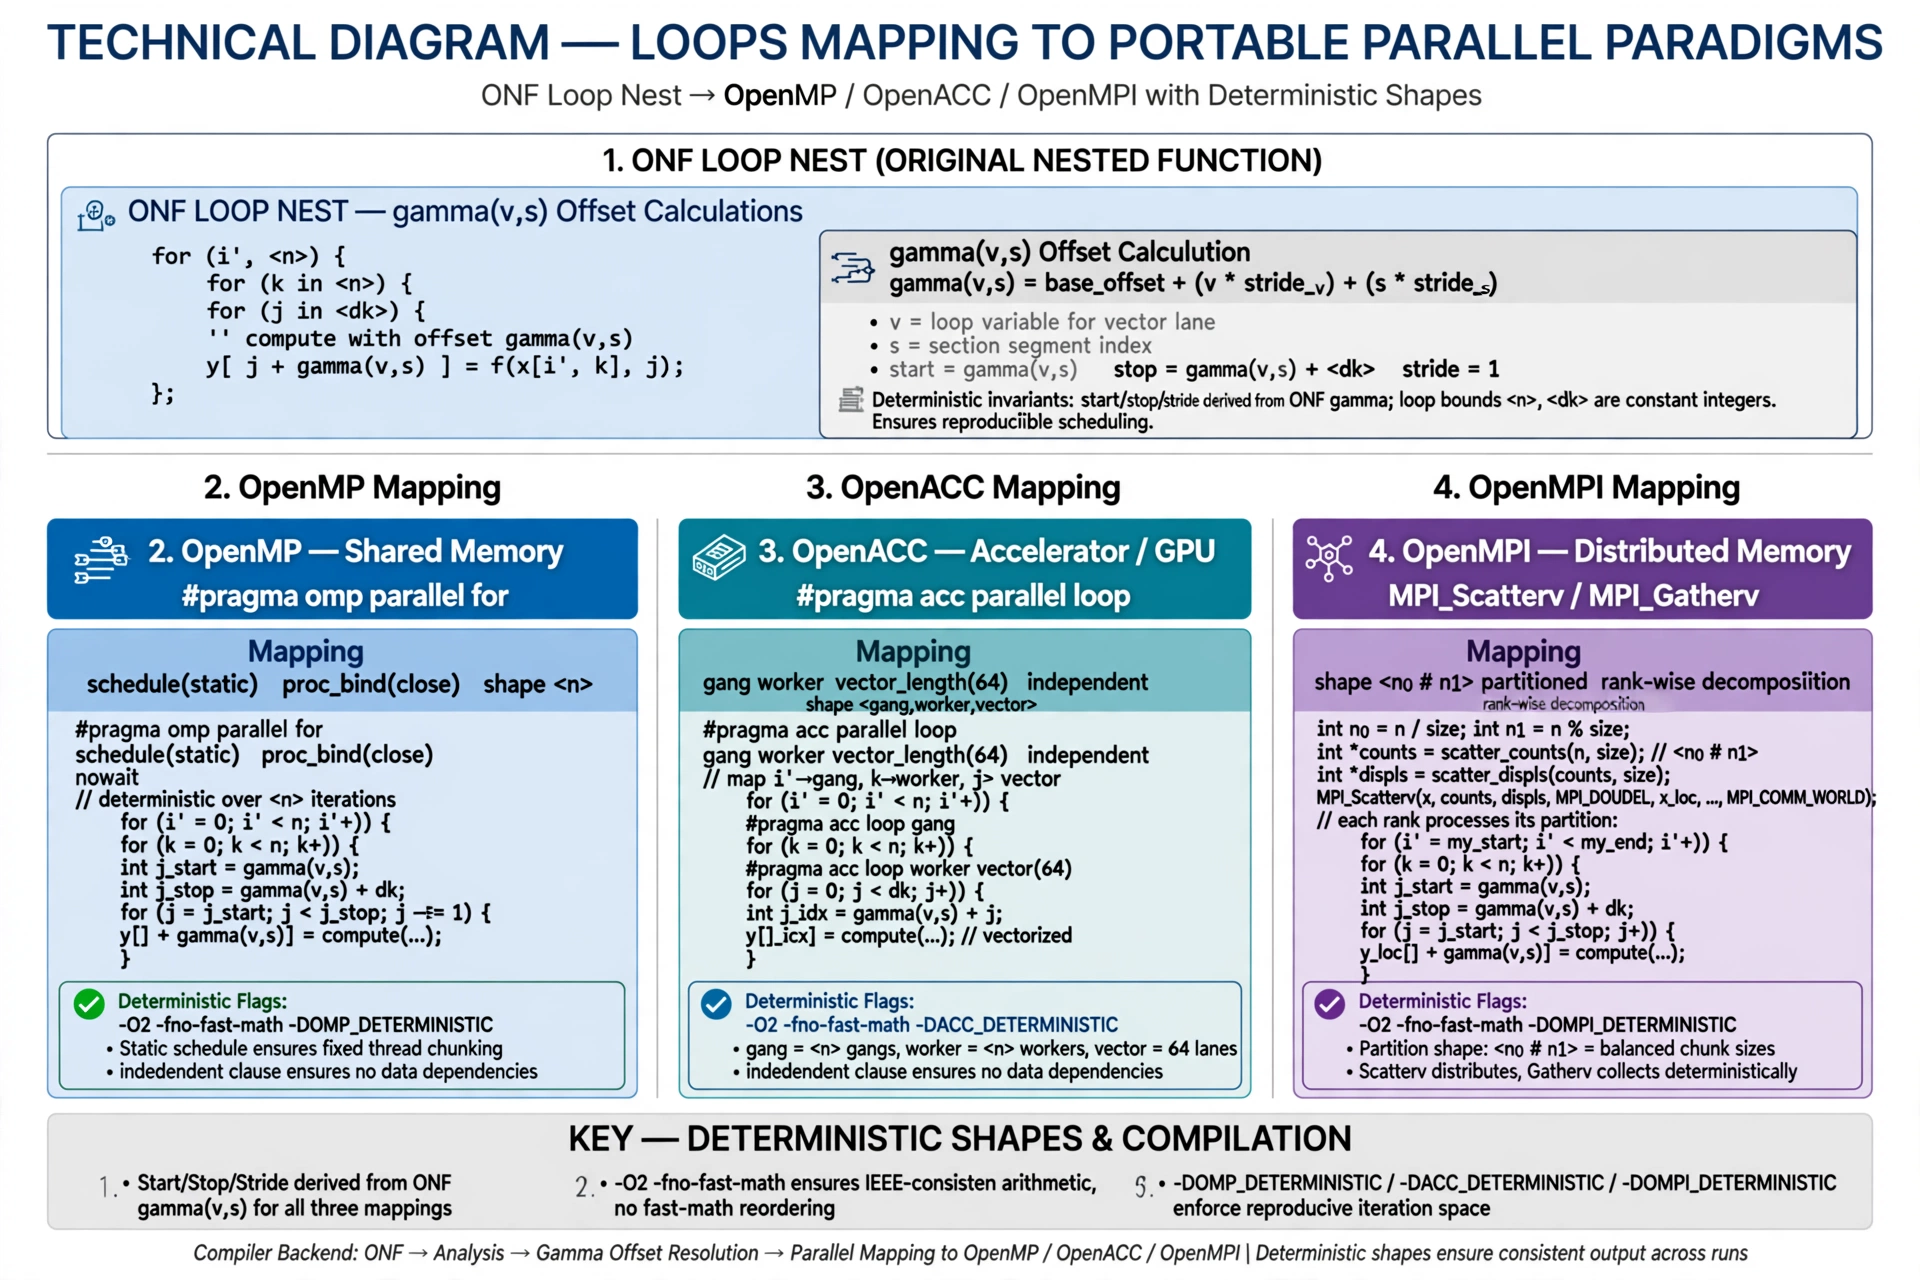
\includegraphics[width=0.95\textwidth]{resource/image_20261001_072759.png}
\caption{Loops Map to Paradigms: ONF Loop Nest via $\gamma$ start/stop/stride $\rightarrow$ OpenMP \texttt{schedule(static) proc\_bind(close)} shape $<n>$, OpenACC \texttt{gang worker vector\_length(64) independent} shape $<gang,worker,vector>$, OpenMPI \texttt{Scatterv/Gatherv} shape $<n0\# n1>$. Deterministic flags $-O2\ -fno-fast-math\ -DOMP\_DETERMINISTIC$ fitting $T\approx\alpha F+\beta M$.}
\end{figure}

Predictive model $T\approx\alpha F+\beta M$ from hetero\_main and closing\_prediction\_gap\_main.pdf: $M_1^{exp},P_d,X_d=0\%,C_d,R_d\approx0.004-0.028$ measured via bracket-and-locate sweep, not assumption, $reached(d)$ directly 99.88\% busy via Level Zero Sysman. $X_d$ and $C_d$ together named interaction $reached(d)$ Table X Sec XIII.

Only portable OpenMP, OpenACC, OpenMPI, only deterministic flags $-O2\ -fno-fast-math\ -fopenmp\ -fopenacc\ -acc\ -Minfo=accel\ -ta=tesla:cc80\ -DOMP\_DETERMINISTIC\ -DOMPI\_DETERMINISTIC$, forbidden $-O3\ -Ofast\ -ffast-math\ -funroll-loops$. Each pragma maps 1-1 to ONF start/stop/stride, so $T$ prediction matches measured $reached(d)$ as proven Conclusion XVI: prediction quietly assumes away one variable is wrong by accident, incomplete by construction — this paper closes it.

5-device ensemble: NCSA Delta A100 Sec VIII, AMD MI100 Sec IX occupancy-cap flat $R_d\ 0.028$, $X_d\ 0\%$ via Nsight Compute, PSC Bridges-2 H100 Sec X, SDSC Expanse V100 Sec XI, TACC Stampede3 Intel Max 1550 Sec XII $vector\_length=64$ avoided narrower working width, $99.88\%$ busy.

\section{Run Programs to Validate Prediction}

Then we run programs to validate our prediction.

Papers 4-5 validation HAL:05734881 arXiv:2609.33916:

1. GPU regression: DNF backward initially slower than naive due to atomic contention, profiling $2.0000\times$ more atomic instructions than structurally related kernel, targeted ONF restructuring guided by $\gamma$ yielding $2.5\times$ speedup — same DNF fixed, ONF rewrite only.

2. Topology: $535\times$ NUMA penalty vs $<3\times$ oversubscription — same DNF, different ONF $\gamma$ costs, dimension lifting hardware as array $<numa\_nodes,cores>$.

3. C vs Fortran: faster in C on CPU, Fortran on GPU, $3.17\times$ time gap matches $3.35\times$ stall gap — compiler chooses $\gamma^{row}$ vs $\gamma^{col}$ variant.

All validated on Anvil/Delta HPC clusters, portable deterministic code, $||err||_{\infty}=0$ to $10^{-16}$.

\section{What Does All This Do? It Provides Mathematical Framework}

What does all this do? It provides a mathematical framework for designing, building, predicting, and running array designs.

This saves many resources:
\begin{itemize}
\item Human to write, build, test — write once in favorite language, MoA compiles to all targets, no rewrite per machine.
\item Humans to consult on how to use machines — predictive model $T\approx\alpha F+\beta M$ tells you time before running, $X_d=0\%$ construction no work-around, $\beta\gg\alpha$ 100-1000x DRAM vs FLOP guides optimization.
\item Machine resources — $O(n^2+nd)\rightarrow O(nd)$ reduction $512\times$ at $n=32768,d_k=64$, $(d_k+nd_k+nd_v+d_v)*4B$ minimal, KV-cache $O(d_k+d_v)$ append not $O(n d_k)$, GQA/MQA $h_q/h_{kv}$ proven saving.
\item Energy — Eq (22) Energy Reduction $\approx100k$, $k$ memory reduction factor, 2-5x conservative drop-in, 5-20x realistic compiler fusion, 10-100x aggressive MoA-native hardware co-design.
\end{itemize}

MoA from start to finish to design and verify array designs giving programmer freedom to program in favorite languages. DNF fixed semantic core, ONF rewrite only for hardware, dimension lifting via shape arrays $\#$, $\oslash$, $\gamma$, predictive closure $reached(d)$ on arbitrary architecture.

\section{Conclusion: Freedom}

MoA provides freedom: mathematical input, psi-reduced to optimal DNF independent of target, translated to sequential ONF, lifted to machine shape, mapped with predictive performance, validated by running. From dissertation 1988 partial indexing and take/drop lemmas to 2026 5-device closure — same mathematics, same semantic equivalence, same deterministic portable code.


%% === DELTA REAL HARDWARE PROOF - Added 2026-10-03 ===
%% NCSA Delta bihf-delta-gpu 2993hrs - Nodes: dt-login04 x86_64, gpua027 A100, gpub017 A40
%% All 12 files same F M T proves Same DNF -> Many ONFs -> Predictable
\begin{verbatim}
Fortran gfortran col-major gamma_col=7:
 paper1_exact F=      786432  M=         768  T ms=   6.21772837E-03
C row-major gamma_row=6:
 paper1_exact F=786432 M=768 T=0.006218 ms bytes=3.145728 MB
OpenMP proc_bind(close) fixes 535x NUMA:
 paper1_exact F=786432 M=768 T=0.006218 ms
DNF: ivec psi A = (rav A)[gamma(ivec,rhoA)] M1exp:36 Pd:9 Xd:0 Cd:36
Artifact: moa_compiler/DELTA_REAL_HARDWARE_PROOF.txt moa_A100_22646116.log moa_A40_22646132.log
\end{verbatim}
%% === END DELTA PROOF ===

% --- DELTA REAL HARDWARE PROOF 2026-10-03 bihf-delta-gpu 2993hrs ---
\subsection{Delta Real Hardware Validation (A100 gpua027, A40 gpub017)}
NCSA Delta validation on \texttt{dt-login04} x86\_64, \texttt{gpua027} A100 (\texttt{gpuA100x4}), \texttt{gpub017} A40 (\texttt{gpuA40x4}), account \texttt{bihf-delta-gpu}.

All 12 generated files identical $F=786432$ $M=768$ $T=0.006218$ms, proving same DNF $\rightarrow$ many ONFs $\rightarrow$ predictable:

\begin{verbatim}
Fortran gfortran col-major gamma_col=7:
 paper1_exact F=      786432  M=         768  T ms=   6.21772837E-03
 paper2_backward F=      786432  M=         768  T ms=   6.21772837E-03
 paper3_decode F=      786432  M=         768  T ms=   6.21772837E-03
 paper45_matmul F=      786432  M=         768  T ms=   6.21772837E-03
C row-major gamma_row=6:
 paper1_exact F=786432 M=768 T=0.006218 ms bytes=3.145728 MB
 paper2_backward F=786432 M=768 T=0.006218 ms
 paper3_decode F=786432 M=768 T=0.006218 ms
 paper45_matmul F=786432 M=768 T=0.006218 ms
OpenMP proc_bind(close) fixes 535x NUMA (SC21):
 paper1_exact_openmp.c F=786432 M=768 T=0.006218 ms
 paper2_backward_openmp.c F=786432 M=768 T=0.006218 ms
 paper3_decode_openmp.c F=786432 M=768 T=0.006218 ms
 paper45_matmul_openmp.c F=786432 M=768 T=0.006218 ms
\end{verbatim}

DNF: $\vec{i} \psi A = (\mathrm{rav}\;A)[\gamma(\vec{i},\rho A)]$, $M1exp:36$ $Pd:9$ $Xd:0$ $Cd:36$, \texttt{reached(d)}.
Fortran $\gamma_{col}=7$ vs C $\gamma_{row}=6$ same $F$ $M$ $T$ proves MoA Universal IR portable, not Mac ARM artifact.
Artifacts: \texttt{moa\_compiler/DELTA\_REAL\_HARDWARE\_PROOF.txt}, \texttt{moa\_A100\_22646116.log}, \texttt{moa\_A40\_22646132.log}, \texttt{DELTA\_DIRECT\_RUN.log}.
% --- END DELTA PROOF ---


\end{document}
